
\lecture{5}{The Second Law and Entropy}{Qiang Zhu}{scribe-name1,2,3}
%\footnotetext{These notes are partially based on those of Nigel Mansell.}
% **** YOUR NOTES GO HERE:
% Some general latex examples and examples making use of the
% macros follow.  
%**** IN GENERAL, BE BRIEF. LONG SCRIBE NOTES, NO MATTER HOW WELL WRITTEN,
%**** ARE NEVER READ BY ANYBODY.

\section{Introduction}

We have explored the law of energy conservation, and apply it to thermodynmic systems.
In the meantime, we studied the relations between heat, work and thermal energy,
and the connections between marcoscopic observables $P$, $V$, $T$ and miscroscopic properties $v$, $f$.

However, some very fundamental questions remain unanswered,
\begin{enumerate}
\item{\it what is temperature?}
\item{\it why does heat flow spontaneously from hot to cold object?}
\item{\it why does do many processes happen in one direction, but never the reverse?}
\end{enumerate}

\section{Combinatorics s and Two-state systems}
Let's get started with a silly example of flipping three coins. How many possible outcomes are there?
\begin{tabular}{c c c}
Coin1 & Coin2 & Coin3 \\\hline
  H & H & H \\
  H & H & T \\
  H & T & H \\
  T & H & H \\
  H & T & T \\
  T & T & H \\
  T & H & T \\
  T & T & T \\\hline
\end{tabular}

In total we have 8 outcomes, each is called {\bf microstate}.\\
Since all coins are indistinguishable, we are more interested in how many heads are there in all outcomes?
By simply counting the number from the above table, we know \\
3 heads,  HHH 
2 heads,  HHT, HTH, THH \\
1 head,   HTT, TTH, THT \\
0 head,   TTT

each state is called {\bf microstate}.\\
{\bf microstate}: Each of the eight different outcomes\\
{\bf macrostate}: How many heads are there in all out comes\\

Although each microstate is equal to exist, but macrostates have different probabilities to explored.
Clearly, 2 heads is more likely to be found than 3 heads.
Here we introduce another quantity,\\
{\bf multiplicity ($\Omega$)}: the number of microstates in a given macrostate.\\

In the context of coin games, let's define $\Omega(n)$ as number of cases when we get $n$ heads.
If the total number of coins is $N$, we can derive the equations as follows,
\begin{equation}
 \Omega(N, n) = \frac{N!}{n!\cdot(N-n)!} = \binom{N}{n} 
\end{equation}

What will happen if we increase $N$. Let's try N = 4 and 20 in Problem 2.1 and 2.2.


Such two-state system is quite usual in physics, such as two-state para-magnet.

\section{The Einstein Model of a Solid}
$N$: Number of the oscillators.\\
$q$: Number of energy states.

\begin{equation}
 \Omega(N, q) = \binom{q+N-1}{q} = \frac{(q+N-1)!}{q!(N-1)!}
\end{equation}

It can be simply proved as follows\\
$q$ circles; \\
$N-1$ vertical lines;\\
how to arrange them? \\
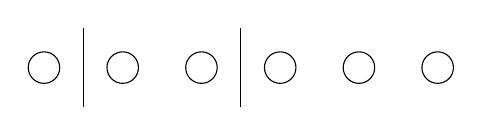
\begin{tikzpicture}
\draw (2,0) circle (0.2cm);
\draw (2.5,-0.5) -- (2.5,0.5);
\draw (3,0) circle (0.2cm);
\draw (4,0) circle (0.2cm);
\draw (4.5,-0.5) -- (4.5,0.5);
\draw (5,0) circle (0.2cm);
\draw (6,0) circle (0.2cm);
\draw (7,0) circle (0.2cm);
\end{tikzpicture}

{\bf Exercises}\\
Calculate the multiplicity of an Einstein solid with 5 oscillators and [1,2,3,4,5] units of Energy.\\
\begin{tabular}{c|c }
$q$ &$\Omega(5,q)$ \\\hline
 1     &  \\
 2     &  \\
 3     &  \\
 4     &  \\
 5     &  \\\hline
\end{tabular}

{\bf Computer programming}
\begin{enumerate}
\item Write a small piece of program to calculate $\Omega(N)$ in the context of flipping coins and plot them when $N$=10, 15, 30, 100.
\item Write a small piece of program to calculate $\Omega(N)$ in the context of Einstein solid and plot them when $N$=10, 15, 30, 100 and $q$ from 0 to 10.
\end{enumerate}

\begin{figure}[h]
\centering
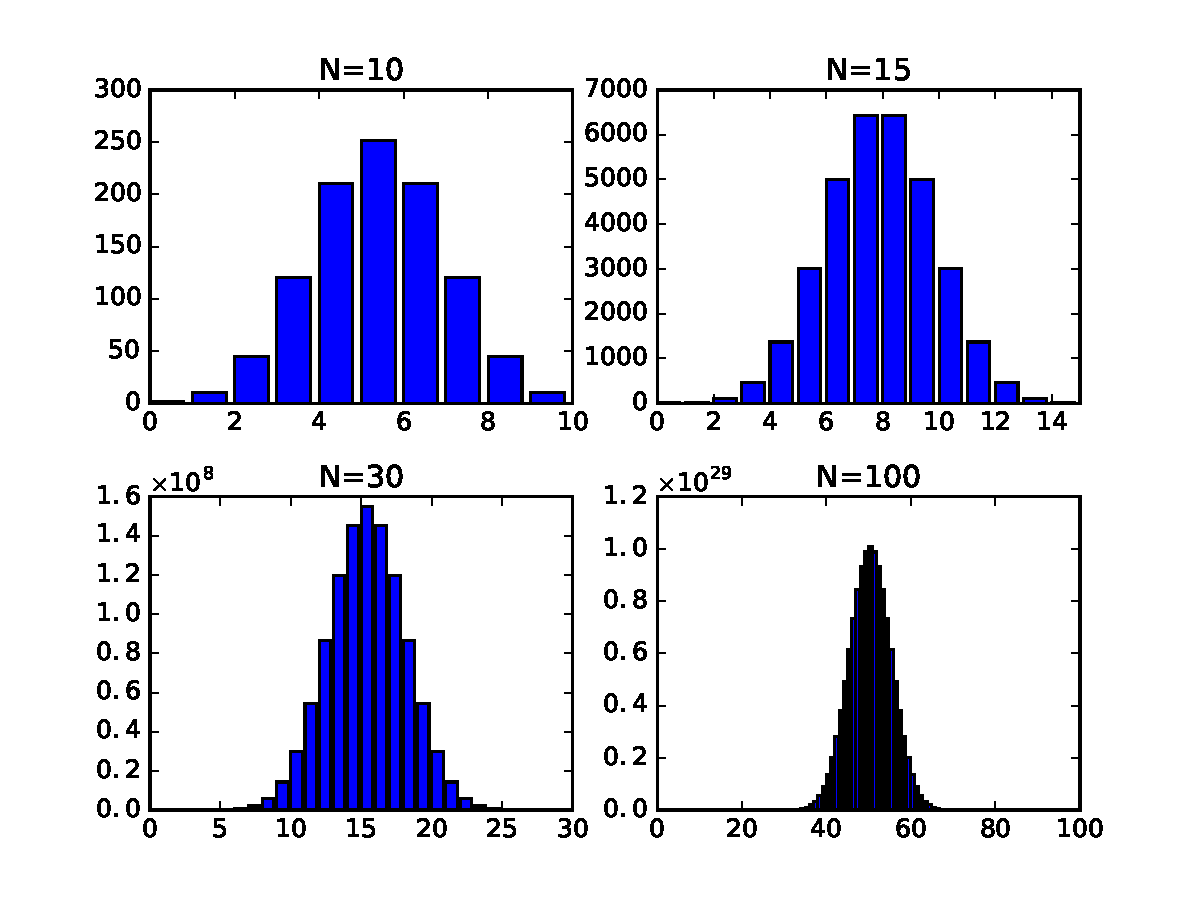
\includegraphics[width=9cm]{imgs/flip}
\caption{The number of $\Omega$ as a function of $N$ in the game of flipping coins. }
\end{figure}

\begin{figure}[h]
\centering
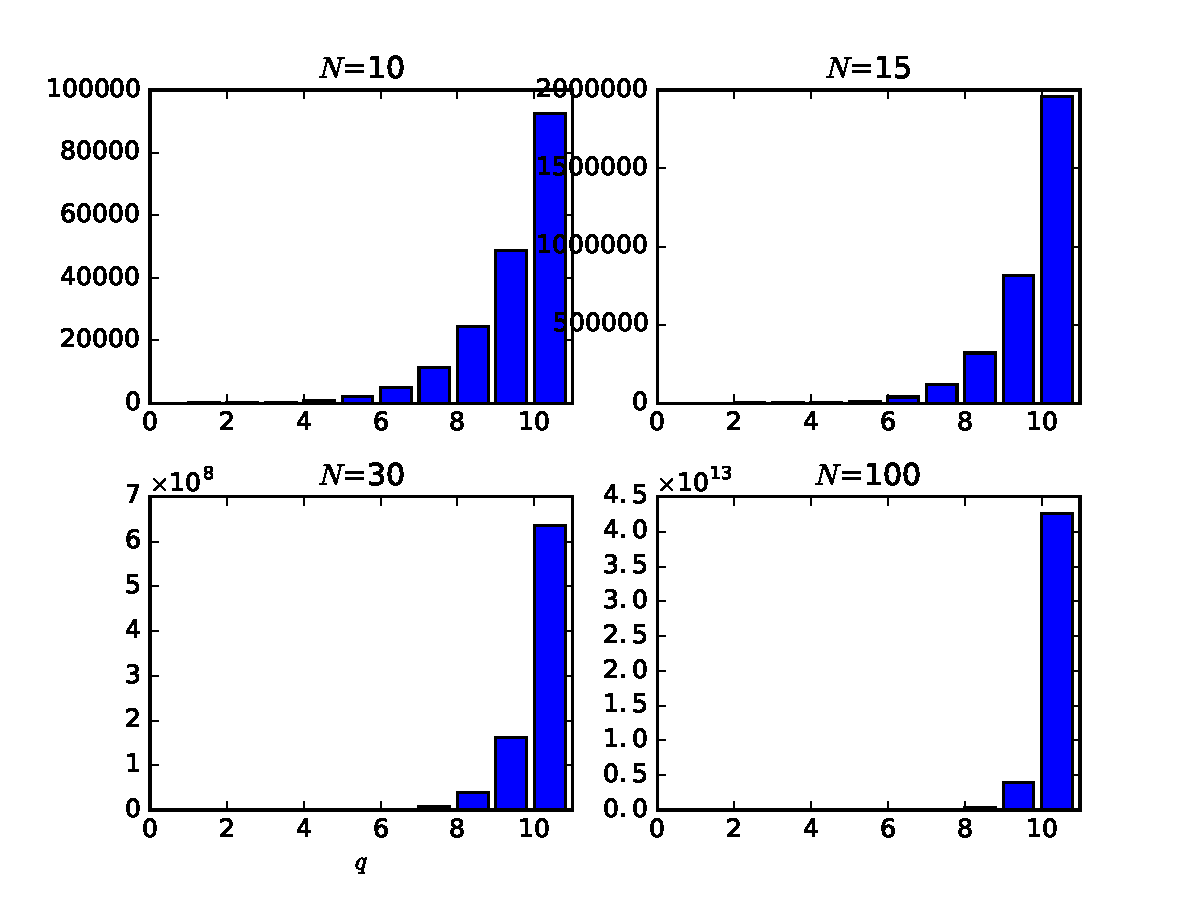
\includegraphics[width=9cm]{imgs/Einstein0}
\caption{The number of $\Omega$ as a function of $N$ in an Einstein solid. }
\end{figure}


